\chapter{Algoritmy na grafoch}
\label{kap:algoritmy}

Táto kapitola obsahuje popisy algoritmov, ktoré sú aplikovateľné na grafové štruktúry a navyše využiteľné pri vyhľadávaní spojení hromadnej dopravy. Formálnu charakterizáciu algoritmu zväčša doprevádza i jeho voľnejšia interpretácia, ktorá má za účel uľahčiť porozumenie čitateľom, ktorí sa s daným algoritmom doposiaľ nestretli. Naviac, pri algoritmoch sú uvedené výhody, respektíve nedostatky, pri jeho použití na nami vytýčený cieľ. V hojnom počte budeme využívať definície z kapitoly \ref{kap:grafy}.

\section{Najlacnejšie cesty v grafe}

Pri vyhľadávaní spojení mestskou hromadnou dopravou sa zdá byť veľmi racionálne zaoberať sa nachádzaním najlacnejších ciest v grafikone MHD. Dovoľujeme si tak tvrdiť, pretože najväčší dôraz cestujúcich je kladený práve na čo najskorší príchod do požadovanej lokality. Pre úplnosť ešte dodávame, že cena cesty, ako je asi zrejmé, je súčet hodnôt hrán (respektíve vrcholov), ktoré daná cesta obsahuje. Z doposiaľ uvedeného vyplýva, že pri našich úvahách budeme používať ohodnotené grafy, kde pridelenou hodnotou bude čas medzi zastávkami. Navyše musíme nejako ošetriť i vrcholy grafu - zastávky, keďže na nich zvyčajne čakáme na prestup na ďalší spoj. Od tejto myšlienky však spočiatku upustíme a budeme sa jej venovať až neskôr. A posledná úvaha - hranami v našom grafe sú linky MHD, sme preto nútení použiť orientované grafy.\newline

Ak uvažujeme vyhľadávanie najlacnejších ciest v grafe, musíme si najprv uvedomiť, čo presne je našim cieľom. Výledok, ktorý chceme dosiahnuť ako výstp algoritmu, má byť najlacnejšia cesta z počiatočného bodu do koncového. Avšak znalosť problematiky algoritmov na grafových štruktúrach nám ponúka riešenia iného, koplexnejšieho problému s asymptoticky rovnakou časovou zložitosťou. Týmto problémom je vyhľadávanie najlacnejších ciest z počiatočného vrcholu do všetkých ostatných vrcholov. Ľahko nahliadnuť, že riešeim tohto problému dostaneme odpoveď aj na našu počiatočnú otázku.  Preto sa v nasledujúcej časti budeme zaoberať algoritmami riešiacimi túto úlohu.\newline

Ľahko spozorovať, že by mohlo byť v určitých situáciách výhodné vypočítať ceny a nájsť najlacnejšie cesty pre všetky dvojice vrcholov. Hlavne, keď graf obsahuje malé množstvo vrcholov - zastávok. Mnoho miest má len malú sieť mestskej hromadnej dopravy, a teda by bolo rozumné vypočítať všetky potrebné údaje naraz na začiatku, a potom, pri prijímaní dotazu na vyhľadanie spojenia, jednoducho vypísať už vypočítanú odpoveď. Z tohto dôvodu uvedieme i algoritmy riešiace tento problém.\newline

\subsection{Dijkstrov algoritmus}

Holandský informatik, po ktorom je tento algoritmus pomenovaný, dokázal, okrem iného, vyriešiť aj nami nastolený problém. V jeho riešení je ale potrebné, aby boli ceny hrán grafu nezáporné reálne čísla, čo súhlasí s našou predstavou aplikovania algoritmu na grafikon MDH. Algoritmus je navrhnutý tak, že dostane ako vstup graf $G = (V, E)$, počiatočný vrchol $v_{0}$ a hodnotiacu funkciu $h: V \times V \rightarrow R^{+}_{0}$. Predpokladáme, že ak hrana $uv \notin E$, potom $h(u,v) = \infty$, ďalej, že $h(u,u) = 0$ a nakoniec, že funkciu $h$ je možné vypočítať v konštantnom čase $O(1)$. Máme taktiež jeden predpoklad na vrcholy grafu, a to, že sú reprezentované celými číslami $1, 2, ..., k$ (kde $k$ je počet vrcholov grafu). Nakoniec, výsledkom algoritmu bude pole čísel $D$, v ktorom bude pre každý vrchol $v \in V$ vypočítaná hodnota $D [v]$, čo je cena najlacnejšej cesty z počiatočného vrchola $v_{0}$ do vrchola $v$. \newline

Tieto požiadavky, predpoklady, ba i vstup a výstup funkcie sú uvažované v horeuvedenom tvare len aby sme mohli predviesť implementáciu algoritmu od Pavla Ďuriša, ktorú možno nájsť aj v jeho knihe \cite[kapitola 2.2.1]{duris2009}.\newline

\begin{algorithm}[H]
  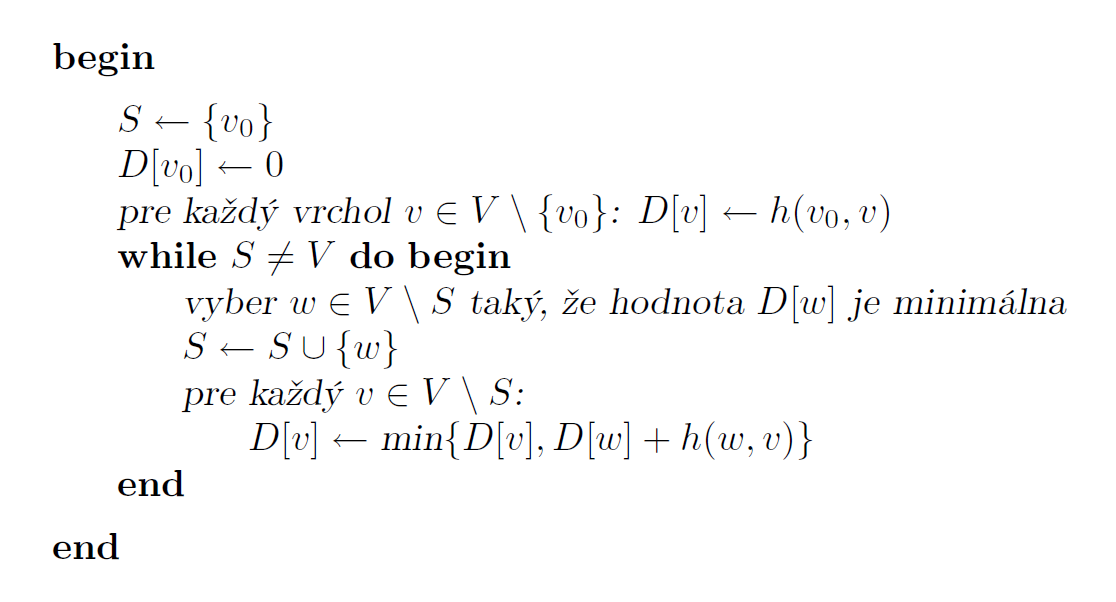
\includegraphics[width=\linewidth]{./images/Alg_Dijkstra.png}
  \caption{Dijkstrov algoritmus}
  \label{Alg_Dijkstra}
  \centering
\end{algorithm}

Časová zložitosť dijkstrovho algoritmu je $O(|V|^{2})$, čo je dokázané spolu s korektnosťou algoritmu v už uvedenom zdroji od Pavla Ďuriša \cite[kapitola 2.2.1]{duris2009}.\newline

Priebeh dijkstrovho algoritmu vysvetlíme na jednoduchom príklade.

\begin{figure}[H]
  \centering{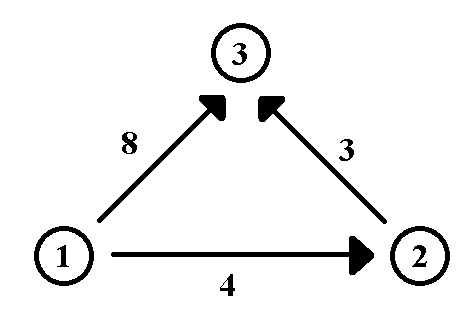
\includegraphics{./images/dijkstra_priklad.png}}
  \caption{Orientovaný graf s ohodnotenými hranami}
  \label{dijkstra_priklad}
\end{figure}

Keďže je našim cieľom nie ani tak zistiť cenu najlacnejšej cesty, ale skôr takéto cesty nájsť, dijkstrov algoritmus by sme potrebovali jemne modifikovať, a to tak, aby sme vedeli spätne zrekonštruovať nájdené cesty. Teda so znalosťou konečného vrchola by sme chceli vedieť vygenerovať postupnosť vrcholov, cez ktoré sme sa do finálneho vrchola dostali. Budeme si preto pamätať pri každom vrchole informáciu, z ktorého vrchola sme sa doň dostali.\newline

Dijkstrov algoritmus sa zdá byť najvhodnejším kandidátom pre účely našej práce. Jeho časová zložitosť je príjemná, implementácia nenánorčná a je dosť ľahké sa v nej orientovať, takže si ju budeme môcť poľahky modifikovať, prispôsobiť našim potrebám. Budeme teda schopný vypísať dodatočné informácie pre používaťeľov aplikácie, prípadne vyhľadávanie spresniť či rozšíriť poďľa jeho potrieb.\newline

\subsection{Bellman - Fordov algoritmus}

\subsection{Floyd - Warshallov algoritmus}

\subsection{Johnsonov algoritmus}